\documentclass[a4paper,10pt]{article}

\usepackage{amsmath,graphicx,fullpage,microtype,hyperref,subfig}%,hypcap}

\DisableLigatures{encoding=*,family=*}
\numberwithin{equation}{section}
\setlength{\parindent}{0px}
\widowpenalty=300
\clubpenalty=300
\hyphenpenalty=300
\hypersetup{colorlinks,citecolor=black,filecolor=black,linkcolor=black,urlcolor=black}

\begin{document}

\label{sec:Cover Page}
\addcontentsline{toc}{section}{Cover Page}

Laurens Bogaardt \hfill \href{http://www.uu.nl/ucu}{University College Utrecht}\\
\href{mailto:L.Bogaardt@students.uu.nl}{L.Bogaardt@students.uu.nl} \hfill SSC 301: Research Project\\
01-07-2011\\

\vspace{4cm}

\begin{center}
\begin{LARGE}
\begin{bf}
The Dynamics of Revelation
\end{bf}
\end{LARGE}
\end{center}

\vfill

\begin{center}
\begin{minipage}[t]{0.7\textwidth}
\begin{bf}
Abstract
\end{bf}
\newline
\newline
In this paper, we will examine the dynamics of Spence's model of costly signalling and will determine under what conditions mixed equilibria emerge. One important finding is that the way in which the pooling strategy is defined, whether its revenue is equal to the high or low one or somewhere in between, will influence whether we see any mixed equilibria within phase space. Another key point is that there are no fundamental differences between dynamics with and without mixed equilibria. In the latter case, these mixed equilibria are simply positioned outside of phase space and we can only observe a small part of a larger dynamic. Lastly, it is suggested that these mixed equilibria may naturally evolve if receivers are allowed to choose the value of their averaged revenue themselves within an infinite strategy space and are maximizing their pay-off. Having established these ideas about costly signalling, this paper continues to examine a variation on the model. Revelation will be included, by which it is meant that senders will not have the option to signal, but must choose whether to fully reveal their type to the receiver or not. It is found that the most likely equilibrium in this case is one in which low quality senders do not reveal when there is a cost associated with this action and high quality senders do reveal their type. Receivers will award their revenues accordingly.
\end{minipage}
\end{center}

\vspace{.4cm}

\begin{center}
\begin{minipage}[t]{0.7\textwidth}
\begin{bf}
Acknowledgements
\end{bf}
\newline
\newline
The author wishes to thank Kris de Jaegher for the supervision during the writing of this paper.
\end{minipage}
\end{center}

\vspace{.6cm}

\newpage

\phantomsection
\label{sec:Contents}
\addcontentsline{toc}{section}{Contents}
\renewcommand{\contentsname}{Contents\\} 
\tableofcontents

\newpage

\section{Introduction}
\label{sec:Introduction}
\subsection{Signalling Theory}
\label{sec:Signalling Theory}

The basic question in signalling theory is the one posed by the sender: "How can I show to the receiver that I am of high quality?". One method of showing this quality is to show that purchasing a certain good is inexpensive for you, because, by assumption, persons with higher quality will pay a lower price for that good. Not all goods will have this negative correlation with quality, so not all goods can act as a signal. By showing that a particular good is inexpensive for you, it follows you must be of high quality. The question then reduces to: "How can I show that this particular good is inexpensive for me?". Standard economic theory suggests that when something is less expensive, you buy more of it; think of the downwards sloping demand curve. So by purchasing more of this particular good, you can show it is not very expensive for you to buy, indicating you are of high quality. Such a signal can be fully informative when, for a person of low quality, it is not worth purchasing the expensive good in order to pretend to be of high quality. The signal, the act of purchasing this particular good, can then perfectly discriminate between high and low quality senders. The signalling of quality can be interpreted in many different ways, with many different 'goods' acting as the signal. One example is that of the peacock who grows a beautiful tail at an expense which is negatively correlated with the quality of the peacock's genes \cite{MaynardSmith2003}. As such, the size, shape and colour of the tail signal the genetic quality of the peacock to the peahen. This example, known as the handicap principle, has been suggested by Zahavi and has been formalised into a model by Grafen \cite{Zahavi1975, Grafen1990}. Another example, particularly important to economics, is the job market signalling model developed by Michael Spence \cite{Spence1973}.

\subsection{Spence's Model}
\label{sec:Spence's Model}

The job market signalling model is quite straight forward. The basic idea follows from the assumption that employers cannot directly observe the quality of the worker they wish to hire. As such, the act of hiring a person is an investment under uncertainty, because employers will need to pay a particular wage but they do not know what the worker's marginal product is. Without full knowledge of the quality, the employer has to make an estimate about the wage to offer. This revenue may be a weighted average based on the available information, such as the average quality of all workers.\\
\\
However, workers may present the employer with another type of information; a signal. In order to obtain a higher wage, the worker purchases a certain level of education to demonstrate his quality. For simplicity, it is assumed that education itself does not alter the worker's quality but is merely a signal. The key point here is that the cost of this signal is negatively correlated with the actual quality of the worker, because higher quality workers will find it easier to go through schooling and obtain a degree. As such, high quality workers may purchase a high level of education at a low cost, while low quality workers would need to spend a lot only to get some level of education. This means that, under the right conditions, employers can distinguish perfectly between those workers with high quality and those with low quality.\\
\\
These basic concepts can be presented more clearly by first making some simplifications. Let us assume there are only two types $\tau$ of senders of signals; high quality and low quality workers. The marginal product of the first group is set to 2 and of the second group to 1. Furthermore, the wage $\rho$ offered to these groups will be exactly their marginal product. Now it remains to be seen how the employer can determine this marginal product. The workers will be able to purchase a certain level of education $\sigma$ at a cost $c(\tau,\sigma)$, where, following the assumption made above, this function is decreasing in $\tau$. In particular, let $c(\tau,\sigma)=\frac{\sigma}{\tau}$ such that the cost of education for low quality workers is equal to the level of education $\sigma$, while for high quality workers it is half this cost, $\frac{1}{2}\sigma$. The employer will then assume that above a particular level of education $S$, all senders are of high quality, while those who purchase less than $S$ are assumed to be low quality workers. This wage schedule, along with the cost functions for the two types of senders, is presented in Figure~\ref{fig:Graph1.png} below.\\

\begin{figure}[h]
\begin{center}
\leavevmode
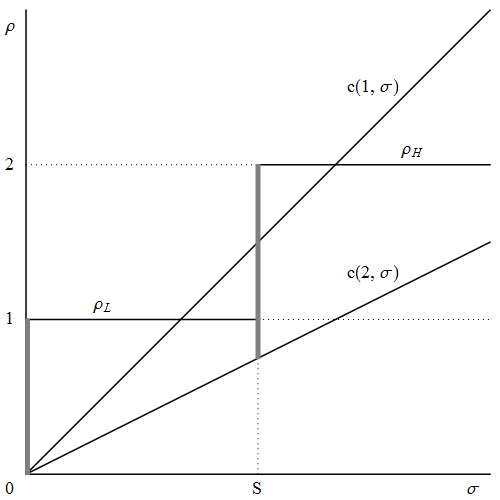
\includegraphics[scale=.4]{Graph1.png}
\end{center}
\caption{Spence's Model}
\label{fig:Graph1.png}
\end{figure}

It is obvious that, in this model, there is no advantage to signalling at a higher level than $S$. Therefore, for those choosing to signal at all, $\sigma=S$ will be their level of education. For those who signal at a lower level than $S$, it is costly to purchase any education at all. This group will signal at $\sigma=0$. Furthermore, following the negative correlation between the quality of the worker with the cost of the signal, it follows that, for the correct value of $S$, the population of senders is perfectly divided into those with low quality who do not signal and those with high quality who signal at level $S$. This is a immediate consequence of profit maximization within the groups of senders as can be seen by the grey lines drawn in Figure~\ref{fig:Graph1.png}. In the present model, this perfect discrimination works only when the employers choose a value of $S$ between 1 and 2. Then, there is no incentive for any player to change their behaviour, or their strategy, and we therefore consider this system to be in equilibrium. In this case, the signal $\sigma$ contains full information about the quality of the sender.

\subsection{Wagner's Model}
\label{sec:Wagner's Model}

The original model by Spence provides a static picture of the equilibrium, even though a mechanism for the dynamics was suggested within the same paper. Dynamics of the signalling game, in which a population of senders and receivers try to find the best strategy to play the game, have been proposed in many other papers, especially in the field of biology when discussing Grafen's model \cite{Cressman2003, Hofbauer1998, Hofbauer2003}. However, few of these extended versions of Spence's model discuss mixed equilibria. The idea that these mixed equilibria, where a proportion of the players plays a certain strategy and a proportion plays a different strategy, are actually prominent in the dynamic version of the model was suggested by Elliot Wagner \cite{Wagner2010}. He showed that under very reasonable values for the model's parameters, mixed equilibria and limit cycles can occur, to which a large proportion of the possible initial population-configurations was attracted. In fact, the boundary face on which the limit cycle occurred attracted more than half of these possible configurations for any value of $S$ \cite{Wagner2010}. It is interesting that few other authors had discussed mixed equilibria to date. A possible reason for this fact will be discussed later on, when we review Wagner's model.\\
\\
It has been suggested that the outcome of costly signalling games may be very counter-intuitive, making them important in explaining odd economic behaviour. These models may not only be applied to economic situations, but they are also key to understanding strange animal behaviour. As Richard Dawkins puts it, animals may taunt predators by making somersaults in front of them if these risks benefit the animal more than they endanger him \cite{Dawkins1976}. A comprehension of the dynamics, then, gives us a better understanding of the methods by which a counter-intuitive equilibrium is reached. To get a full understanding of the dynamics of signalling games and the existence of mixed equilibria it is, therefore, important to investigate Wagner's model carefully. This will be done in Section~\ref{sec:The Dynamics of Costly Signalling} after having gone over the basics of signalling games in Section~\ref{sec:The Basic Action-Response Model}. The model will then slowly be built up, allowing us to tweak the values of the model's parameters to see what effects this would have. After having reviewed the existing literature on costly signals and after having examined under what conditions mixed equilibria appear, a variation of the model will be made. Senders can always lie by signalling dishonestly and signals can always be disbelieved by the receiver. However, in some situations, a sender may choose to fully reveal his type, i.e. to show whether he is of high or of low quality. The model by Wagner can be altered slightly to be interpreted as a revelation model. As far as we know, this sort of variation has not been attempted yet. We will see that the same type of dynamics results, which will be presented in Section~\ref{sec:Variation on the Model}. Finally, it will be important to interpret both the results of the investigation into Wagner's model as well as the merit of the variation on his model. This is done in Section~\ref{sec:Conclusion}.

\section{Replication of the Model}
\label{sec:Replication of the Model}
\subsection{The Basic Action-Response Model}
\label{sec:The Basic Action-Response Model}

The most basic and generic signalling model is the basic action-response model, also called the basic signalling game, in which there are two players, the sender and the receiver \cite{Hurd1995, Fudenberg1991}. The sender can be one of two types $\tau$; either he has high quality with $\tau=H$ or he has low quality with $\tau=L$. The probabilities for these two cases are $P_H$ and $P_L$, respectively. Clearly $P_H+P_L=1$. Furthermore, the sender can send a signal $\sigma$ where he has the choice between signalling east or west, $\sigma=E$ or $\sigma=W$. The receiver then has the choice to assign the sender a revenue $\rho$, previously in the job market signalling model called wage, which is up or down, either $\rho=U$ or $\rho=D$.

\begin{figure}[h]
\begin{center}
\leavevmode
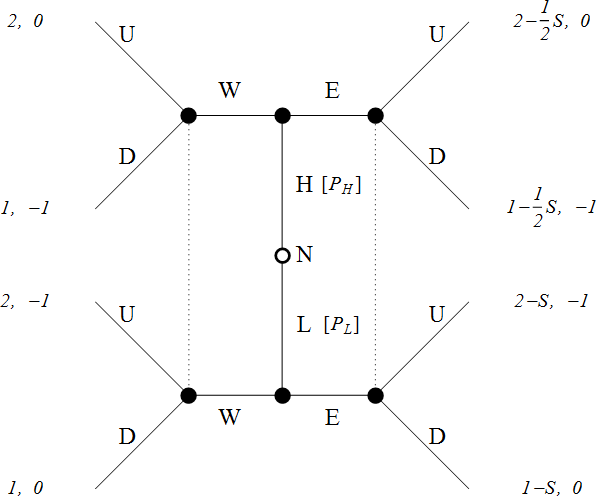
\includegraphics[scale=.4]{Graph2.png}
\end{center}
\caption{The Basic Action-Response Model}
\label{fig:Graph2.png}
\end{figure}

The model described above is presented in the extensive form in Figure~\ref{fig:Graph2.png}. It can be seen that the two types of senders have two choices in signalling, and that the receiver has two choices in his action, resulting in eight possible states. In accordance with the original model by Spence, as well as Wagner's model, the pay-off to the players is determined by the type of sender, the signal and the awarded revenue. In particular, we again have senders who have a marginal product of either 1 or 2 and who are, therefore, awarded a revenue $\rho$ equal to either 1 or 2. They also incur a cost of signalling $c(\tau,\sigma)=\frac{\sigma}{\tau}$. Furthermore, we have a receiver who pays the sender the revenue and receives their marginal product in return. It will be assumed that the receivers do not necessarily wish to minimize costs, but that they want to pay the senders their marginal product accurately. An interpretation of this assumption in the job market is that employers wish to pay the workers just enough so that they are not hired by the competition \cite{Gibbons1992}. This means that they want to minimize the difference between the revenue they pay and the marginal product they receive. This can be parameterised by assuming the pay-off to the receiver is $-{(\tau-\rho)}^2$. Following these assumptions, we obtain the values given in the basic action-response model above.

\subsection{Infinite Strategy Space}
\label{sec:Infinite Strategy Space}

One limitation of the basic action-response model is that the revenue paid by the receiver is limited to either Up or Down. Although there are more simplifications used to be able to model the dynamics properly, this one is particularly restrictive. For example, if a receiver chooses not to believe any signal, what revenue does he pay the sender? In that case, he would award both types of senders an equal revenue; in Figure~\ref{fig:Graph1.png}, this corresponds to a wage schedule which is constant for all $\sigma$, somewhere between $\rho_D$ and $\rho_U$. Most accounts of such a situation, in which the receiver pools the low signallers and high signalling into one group, allow the receiver to pay the sender either a revenue $\rho_D$ or $\rho_U$, in our case 1 or 2. However, it makes little sense that the receiver would pay either this too low a revenue or a much too high a revenue to the pooled group of low and high quality senders. Paying an averaged revenue, somewhere between $\rho_D$ and $\rho_U$ makes more sense. In particular, let $\rho_D<\rho_A<\rho_U$, where $\rho_A=1+K$ with $0<K<1$; we then arrive at the extensive form game presented below in Figure~\ref{fig:Graph3.png}. This is very similar to an infinite strategy space. However, here we will not allow the individual receiver to decide on the value of the parameter $K$, but we will set it globally for all receivers ourselves, restricting the options for the receivers to three; Up, Average and Down, paying the senders either $\rho_U$, $\rho_A$ or $\rho_D$. It should be noted that when $K=P_H$, the game reduces to Wagner's model, presented in Figure~\ref{fig:Graph4.png}. Wagner assumed that, when choosing for the pooling strategy, the receivers would pay an averaged revenue which was equal to the expectation of the marginal product they would receive, resulting in $\rho_A=1 P_L+2 P_H = 1+P_H$. This assumption is very reasonable, but for our discussing we wish to see what happens when we allow $\rho_A$ to vary.

\begin{figure}[h]
\begin{center}
\subfloat[Extensive form of infinite strategy space]{\label{fig:Graph3.png}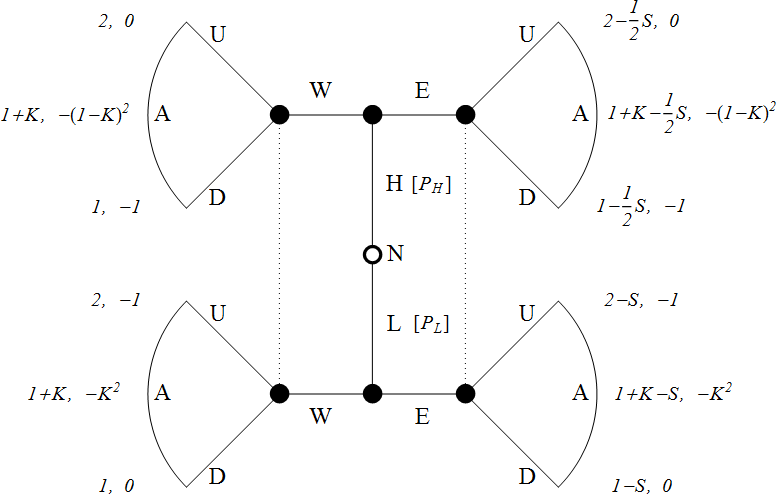
\includegraphics[scale=.305]{Graph3}}
\hfill
\subfloat[Extensive form of Wagner's model]{\label{fig:Graph4.png}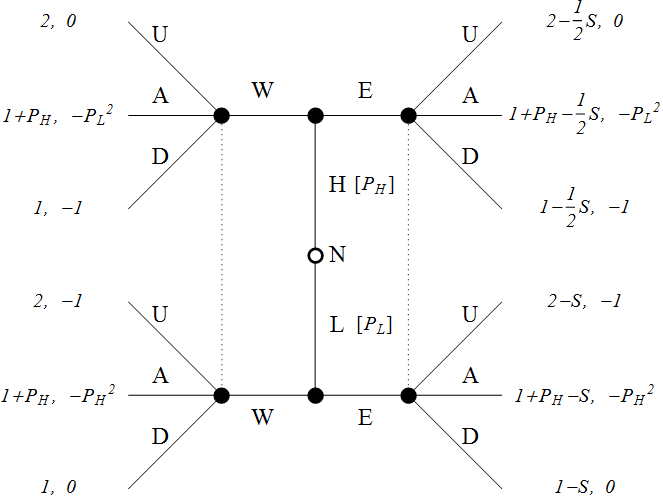
\includegraphics[scale=.305]{Graph4}}
\end{center}
\caption{Extensive forms of the signalling models}
\label{fig:Graph3.png and fig:Graph4.png}
\end{figure}

\subsection{Pruning and Nash Equilibria}
\label{sec:Pruning and Nash Equilibria}

We have already discussed that senders will not choose to signal above $S$ because there is no benefit while there is an additional cost. Similarly, for those senders who signal below $S$, there is no advantage to signal at all. This meant we were able to reduce the complexity of the game to such a degree that it could be depicted in the extensive forms like the ones above.\\
\\
Following the extensive forms in Figure~\ref{fig:Graph3.png and fig:Graph4.png}, the senders have four strategies they can play. As a response to their type $\tau$, they can either signal east at $\sigma=S$ or west at $\sigma=0$. The receivers have more strategies to play. They can respond differently to different signals and have nine strategies in total, depicted in Table~\ref{tab:Strategies} below.\\

\begin{table}[h]
\begin{center}
\begin{tabular}{c|c|ccc|c|c}
\multicolumn{2}{c|}{Response to}&Name& \hspace{1.5cm} &\multicolumn{2}{c|}{Response to}&Name\\
High&Low&&&East&West&\\
\cline{1-3}
\cline{5-7}
&&&&&&\\[-.3cm]
E&E&High&&U&U&Always Up\\
E&W&Separating&&U&A&Split-Up\\
W&E&Anti-Separating&&U&D&Split\\
W&W&Low&&A&U&Anti-Split-Up\\
\multicolumn{3}{c}{}&&A&A&Always Average\\
\multicolumn{3}{c}{}&&A&D&Split-Down\\
\multicolumn{3}{c}{}&&D&U&Anti-Split\\
\multicolumn{3}{c}{}&&D&A&Anti-Split-Down\\
\multicolumn{3}{c}{}&&D&D&Always Down\\
\end{tabular}
\end{center}
\caption{Strategies of the senders and receivers}
\label{tab:Strategies}
\end{table}

However, not all of these strategies make sense and it is possible to simplify our model by ignoring some of them, without much loss of generality. It is easy to see that the strategy Anti-Separating is not very appropriate for senders. In that case, low quality senders would signal at a high cost, while high quality senders, who could potentially signal at a low cost, would not do so at all. Therefore, we will assume no sender will choose this strategy and we remove it from the list. The receivers have a lot of strategies to choose from, however, we can follow the previous line of argument and remove all Anti- strategies, because it seems unreasonable for a receiver to assume that high signals actually come from the low quality senders, while no signal would indicate a high quality sender. Furthermore, we notice the strategies Always Up, Always Average and Always Down are fundamentally the same. In these cases, the receiver would ignore the signal completely, i.e. he would pool the high and low senders together, and would pay everyone an equal revenue. Again, without loss of generality, we can remove the strategies Always Up and Always Down, and keep Always Average as a reasonable pooling strategy. In fact, having defined Average the way we did, we can obtain a wage anywhere from Up to Down by varying our parameter $K$ from 0 to 1. Finally, the three Split- strategies are really also one fundamental strategy in which a high signal will be awarded a higher revenue. As such, Split-Up and Split-Down are removed and we are left with only two strategies for the receiver, together with the three strategies for the sender. It then follows that there are exactly six combined strategies for the senders and the receivers, as are depicted in Table~\ref{tab:PayoffMatrix3D1} below.

\begin{table}[h]
\begin{center}
\[
\begin{array}{r|c|c}
& \text{Average} & \text{Split}\\
\hline
&&\\[-.3cm]
 \text{High} & 
\begin{array}{ll}
\hspace{3.6cm} & -P_H (1-K)^2-P_L K^2 \\
 1+K-\frac{1}{2}P_H S-P_L S& 
\end{array}
 & 
\begin{array}{ll}
\hspace{3cm} & -P_L \\
 2-\frac{1}{2}P_H S-P_L S& 
\end{array}
\\
 \text{Separating} & 
\begin{array}{ll}
\hspace{3.6cm} & -P_H (1-K)^2-P_L K^2 \\
 1+K- \frac{1}{2}P_H S & 
\end{array}
 & 
\begin{array}{ll}
\hspace{3.6cm} & 0 \\
1+P_H-\frac{1}{2}P_H S & 
\end{array}
 \\
\text{Low} & 
\begin{array}{ll}
\hspace{3.6cm} & -P_H (1-K)^2-P_L K^2 \\
 1+K &
\end{array}
 & 
\begin{array}{ll}
\hspace{3cm} & -P_H \\
 1 & 
\end{array}
\end{array}
\]
\end{center}
\caption{Pay-off matrix of the infinite strategy space}
\label{tab:PayoffMatrix3D1}
\end{table}

The pay-off matrix above is based on certain game dynamics. We will assume that there is a population of infinitely many senders and receivers. In every iteration of the game, each sender is randomly assigned to a receiver and plays the signalling game. They will each be awarded a pay-off as given by the extensive form in Figure~\ref{fig:Graph3.png}, limited by the strategies they are allowed to play. Within this game mechanism, the expected pay-off for each strategy can be determined. An explicit calculation will be given in the appendix, Section~\ref{sec:Pay-Off Matrix Calculations}, which shows how to obtain the values in the pay-off matrix above.\\
\\
Having established these pay-offs, we can see which combined strategies are Nash equilibria. When the receiver plays Average, the best strategy for the sender is Low. This is true for any value of $P_H$, $P_L$ and $S$; remember that is follows from the definition of $S$ that it is always greater than 0. When the sender plays Low, the receiver gets the largest benefit from choosing the Average strategy under the most reasonable values of $P_H$ and $K$. More precisely, when $K<2 P_H$, (Low, Average) is a Nash equilibrium. We also see that only when the sender is playing Separating, does the strategy Split become most favoured by the receiver. The (Separating, Split) combined strategy becomes a Nash equilibrium when there is also no incentive for the sender to change strategy. This happens when the pay-off $1+P_H-\frac{1}{2}P_H S$ is greater than both 1 and $2-\frac{1}{2}P_H S-P_L S$. Only for values of $1<S<2$ does this hold. We will then have two pure Nash equilibria in this model. There may, however, be other mixed Nash equilibria. Mixed equilibria occur when part of the infinite population of senders or receivers play one strategy, while others plays a different strategy. In particular, let $x_1$, $x_2$ and $x_3$ be the proportions of senders who play strategies Low, Separating and High, respectively. Furthermore, let $y_1$ and $y_2$ be the proportions of receivers who play Average and Split, respectively. Clearly, $x_1+x_2+x_3=1$ and $y_1+y_2=1$. A mixed equilibrium then occurs when, for a particular ratio of different strategies, there is no incentive for any player to change his behaviour. Whether these mixed equilibria really occur, and for what values of the model's parameters, will be discussed in combination with the dynamics of the model.

\subsection{The Dynamics of Costly Signalling}
\label{sec:The Dynamics of Costly Signalling}

Dynamics will be added to this costly signalling model by means of the replicator equation. The replicator equation was originally devised to simulate evolution by natural selection \cite{Taylor1978}. The replicator equation describes how, in an infinite population of players with different strategies, those players with more successful strategies will grow in number, while the less successful players may be driven to extinction. More details on the replicator equation will be given in the appendix, Section~\ref{sec:The Replicator Equation}. It is easy, however, to reinterpret these dynamics as one of a process of learning and imitation \cite{Vega-Redondo2003}. In that case, the replicator equation describes an infinite population of players of a particular game who have the choice between strategies and who are able to see which strategy is more successful globally. In every new iteration of the game, a proportion of the players adjusts its strategy to the more successful one. In our case, we have a population of senders and of receiver. As already discussed, the first group is divided into three subgroups, $x_1$, $x_2$ and $x_3$, while the receivers consist of subgroups $y_1$ and $y_2$. As the proportions for our groups add up to 1, we can present the configuration of our population in a simplex, which reduces the degrees of freedom for each group by one. The full state of the model is then given in a three dimensional phase space.\\
\\
As the three dimensional phase space of the signalling model may still be complicated to analyse, we will start by looking at the two dimensional case when we limit the strategies of the sender to either Separating honestly or to sending the Low signal $\sigma=0$. This is equivalent to examining one boundary face of the three dimensional phase space, for which $x_3=0$. The strategies for the receiver will be the Average option, i.e. to pay a revenue equal to $1+K$, or to Split the revenue honestly and pay 1 for low senders and 2 to high senders. By varying the parameter $K$, we can then examine the effect of this Average option on the equilibria of the system.

\begin{figure}[h]
\begin{center}
\subfloat[$K=0$]{\label{fig:Graph7.png}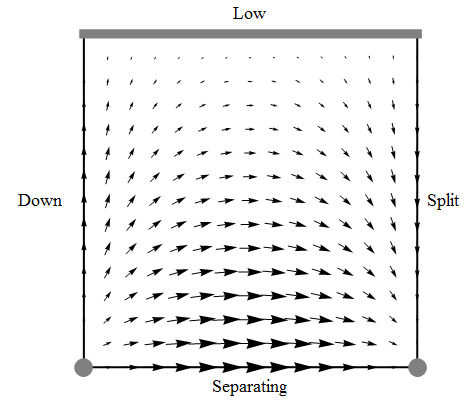
\includegraphics[scale=.19]{Graph7}}
\hfill
\subfloat[$K=.1$]{\label{fig:Graph8.png}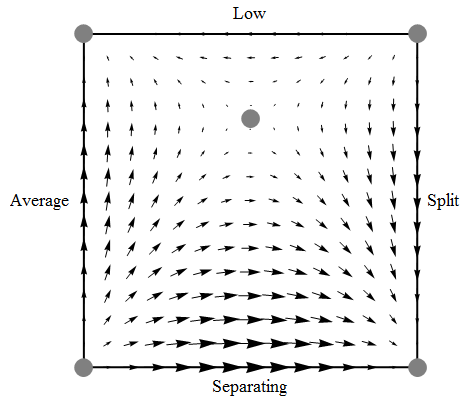
\includegraphics[scale=.19]{Graph8}}
\hfill
\subfloat[$K=.5$]{\label{fig:Graph9.png}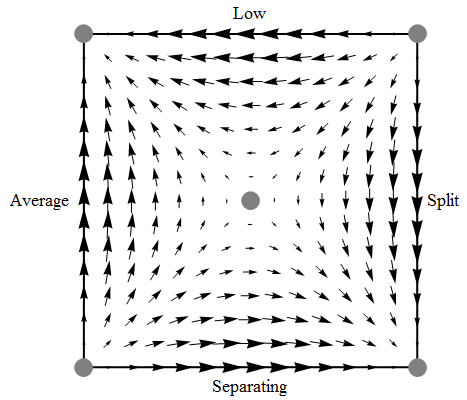
\includegraphics[scale=.19]{Graph9}}
\hfill
\subfloat[$K=.9$]{\label{fig:Graph10.png}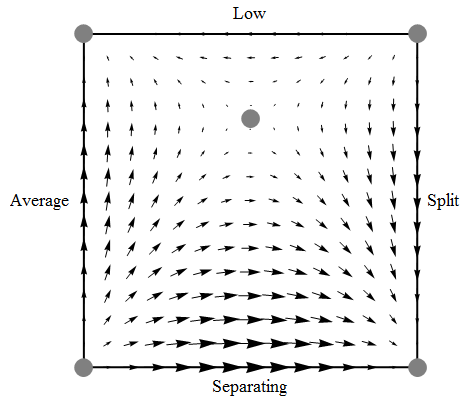
\includegraphics[scale=.19]{Graph10}}
\hfill
\subfloat[$K=1$]{\label{fig:Graph11.png}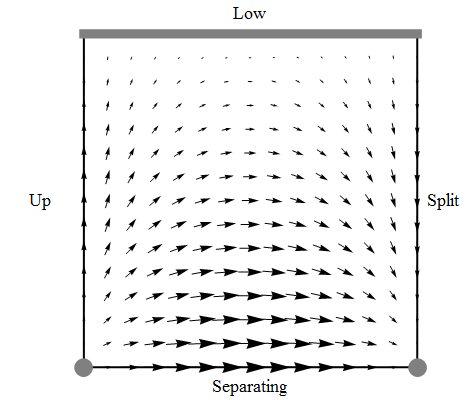
\includegraphics[scale=.19]{Graph11}}
\end{center}
\caption{Phase space for increasing values of $K$ with $S=1$ and $P_H=.5$}
\label{fig:Graph7.png, fig:Graph8.png, fig:Graph9.png, fig:Graph10.png and fig:Graph11.png}
\end{figure}

In the graphs above, it can be seen that for $K=0$, when the receiver pays the low revenue $\rho=1$ to all senders, there is no mixed equilibrium. However, the boundary of phase space when all senders do not signal is neutrally stable. If $P_H=P_L$, as in our case, this same goes for the situation with $K=1$, when the receiver pays the high revenue $\rho=2$. In between, however, a mixed equilibrium appears. In fact, this is a saddle point from which the dynamics lead to either the (Low, Average) equilibrium or to the (Separating, Split) equilibrium. It turns out that the mixed equilibrium is located at a position in phase space where the ratio of the senders' and receivers' strategies depend on the parameters $P_H$, $S$ and $K$. The exact calculations for these values are given in the appendix, Section~\ref{sec:Mixed Equilibria}.

\begin{subequations}
\label{eq:Position2D-1}
\begin{equation}
x_1=\frac{{K}^2+P_H-2 {K} P_H}{P_H}
\end{equation}
\begin{equation}
y_1=1-\frac{1}{2}S
\end{equation}
\end{subequations}

As can be seen from these coordinates, when $K=0$, the mixed equilibrium moves to the edge of phase space where every sender plays Low. The dynamics, as seen in Figure~\ref{fig:Graph7.png}, looks fundamentally different from the one with the mixed equilibrium, but it is not. The part we see within phase space is only one section of the dynamics of the situation with the saddle point, the lower half in the case of Figure~\ref{fig:Graph9.png}, because the saddle point itself has shifted upwards beyond the upper boundary of phase space. Previous accounts of the signalling model often included a pooling strategy in which the receivers paid the low and the high signallers an equal revenue of either $\rho=1$ or $\rho=2$. As can be seen from the graph above, for these values there is no mixed equilibrium, at least, not within the boundaries of phase space. It is, therefore, understandable why mixed equilibria where often overlooked and why Wagner's model, which included a pooling strategy with an averaged revenue of $1+P_H$, seems to be one of the few accounts of mixed equilibria. One more point that should be noted is that when $K=P_H$, the x-position of the saddle point simplifies to $P_L$, the same values found by Wagner \cite{Wagner2010}.\\
\\
We have now looked at one boundary face of the three dimensional signalling model and have established the conditions for the existence of a mixed equilibrium. There is another boundary face which is interesting to examine. This is the one for which $x_1=0$, when we limit the strategies of the sender to either Separating honestly or to sending the High signal $\sigma=S$ .
 
\begin{figure}[h]
\begin{center}
\subfloat[$K=0$]{\label{fig:Graph12.png}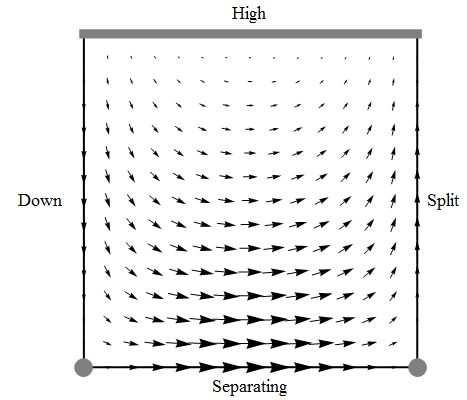
\includegraphics[scale=.4]{Graph12}}
\hfill
\subfloat[$K=.5$]{\label{fig:Graph13.png}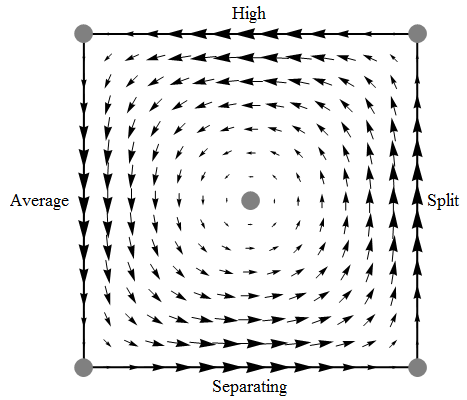
\includegraphics[scale=.4]{Graph13}}
\end{center}
\caption{Phase space for two values of $K$ with $S=.5$ and $P_H=.5$}
\label{fig:Graph12.png and fig:Graph13.png}
\end{figure}

As can be seen in the graphs above, we again find that the mixed equilibrium appears only within the boundaries of phase space for particular values of the parameters $P_H$, $S$ and $K$. Had the Average option been limited to only represent a pooling revenue of either $\rho=1$ or $\rho=2$, the mixed equilibrium would not have appeared within phase space and one would have concluded it did not exist.

\begin{subequations}
\label{eq:Position2D-2}
\begin{equation}
x_3=\frac{K^2+P_H-2 K P_H}{P_L}
\end{equation}
\begin{equation}
y_1=1-S
\end{equation}
\end{subequations}

In the case of this boundary face, the mixed equilibrium is a stable limit cycle. When the senders who play High are more numerous, it becomes advantages for the receivers to play Average. However, then the incentives for the senders switch and they start to play Separating more. This will cause the receivers to choose Split, finally giving the senders a reason to return to their original strategy High. The mixed equilibrium, in this case, is not attracting. However, as can be seen in Figure~\ref{fig:Graph12.png}, when the boundary High is neutrally stable, the part closest to (High, Split) becomes attractive taking in all of phase space's initial conditions. We also see from Equations~\ref{eq:Position2D-2} that the mixed equilibrium moves completely beyond the Split boundary when $1<S<2$. As can be seen in the graph below, in that case (Separating, Split) becomes a Nash equilibrium which attracts all of phase space.

\begin{figure}[h]
\begin{center}
\leavevmode
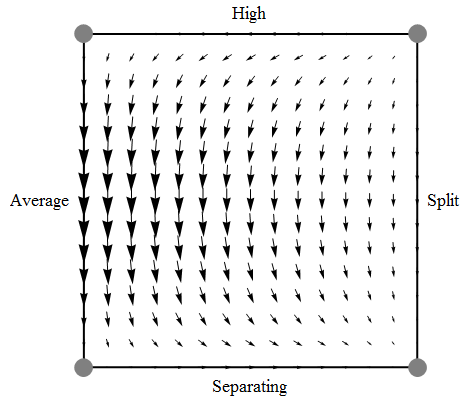
\includegraphics[scale=.4]{Graph14.png}
\end{center}
\caption{Phase space for $K=.5$, $S=1.5$ and $P_H=.5$}
\label{fig:Graph14.png}
\end{figure}

As was discussed, we have only been looking at boundary faces for which certain strategies were disallowed. The dynamics may also be presented in a three dimensional phase space, where the above strategies are put together.

\begin{figure}[h]
\begin{center}
\leavevmode
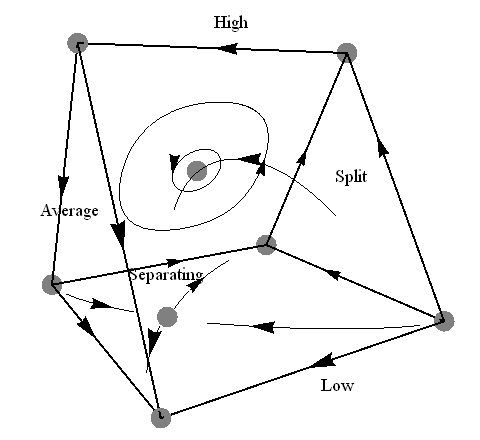
\includegraphics[scale=.75]{Graph15.png}
\end{center}
\caption{Three dimensional phase space with $K=.5$, $P_H=.5$ and $S=.5$.}
\label{fig:Graph15.png}
\end{figure}

As was to be expected, we again see the saddle point and the limit cycle appearing for values of the parameters which give us these mixed equilibria. In this case, the boundary face on which the limit cycle occurs attracts more than half of phase space \cite{Wagner2010}.

\section{Variation on the Model}
\label{sec:Variation on the Model}
\subsection{Revelation}
\label{sec:Revelation}

The model by Wagner allows easily for a variation. In particular, it would be interesting to include revelation; a concept which, we believe, has not yet been explored in this manner. Revelation is the full disclosure of one's type, i.e. the sender will have the choice to either hide his quality to the receiver or to show him exactly what type he is. A possible example of a situation of revelation is a salesman who is selling a good. In doing so, he may use the strategy of letting his customers try out the good before buying it. As such, he can reveal the actual quality of the good to the buyer, who then has full information about how much the good is worth. Of course, the salesman may also choose not to reveal the quality of his good. Then the buyers will not have full information about its quality. However, as we will see, it may turn out that the act of hiding the good's quality, by not revealing it, also sends important information to the buyer. The reason Wagner's model is perfect for this concept is that in revelation lying is not possible. As such, the model is by default already pruned to include only a few reasonable strategies.

\subsection{The Extensive Form}
\label{sec:The Extensive Form}

In accordance with the basic action-response model and with Wagner's model, senders will be of either two types, high or low quality. They will have the choice to reveal their type or to hide it. It therefore makes sense to consider $\sigma=0$ as not revealing and $\sigma=1$ as revealing. Revelation also potentially brings about a cost to the sender. In this case, the act of revealing is equal to both high and low quality senders. Therefore, the cost will also be equal, i.e. it will be independent of the type $\tau$. Furthermore, as revealing is a yes or no option, the cost will also simply be a constant and not a function of $\sigma$. Let us call the cost of revealing $C$. Furthermore, the receiver can pay the sender a revenue which is either Up or Down, or an Average. The extensive form of this model is presented below in Figure~\ref{fig:Graph5.png}.

\begin{figure}[h]
\begin{center}
\leavevmode
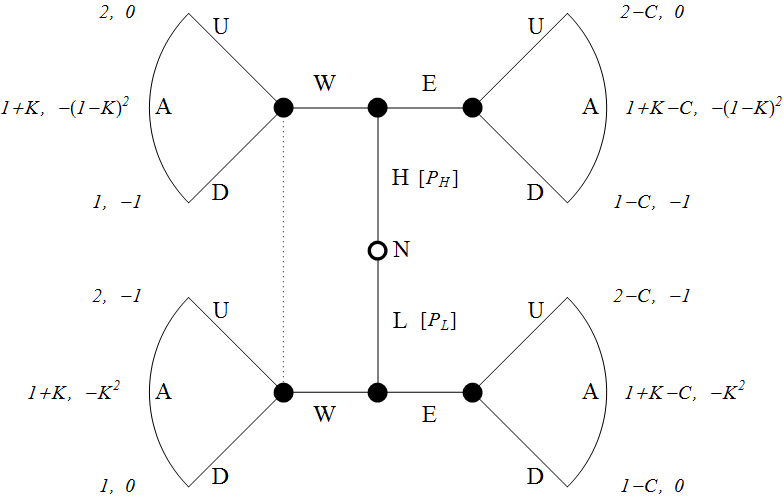
\includegraphics[scale=.4]{Graph5.png}
\end{center}
\caption{Extensive form for the revelation model}
\label{fig:Graph5.png}
\end{figure}

\subsection{Pruning and Nash Equilibria Again}
\label{sec:Pruning and Nash Equilibria Again}

Just like with the signalling model, the revelation strategy space needs to be pruned first. This is again done to simplify matters, hopefully without loss of too much generality. It turns out that pruning is even easier for the revelation model. As was already mentioned, in the signalling model, low quality senders may lie and pretend to be of high quality by signalling like a high quality sender. However, in the revelation model, a sender who has revealed his type to the receiver is out of options. There is no pretending possible as the receiver sees the quality of the sender as it is. Out of all the strategies for the receiver, then, only a few are reasonable for examination. Some of the strategies are given below in Table~\ref{tab:StrategiesRevelation}. The full list of all the strategies for the receiver is given in the appendix, Section~\ref{sec:The Strategies for Revelation}. For the sender, the same strategies as in the signalling model remain, however, the strategies Low and High now simply have a different interpretation meaning Never Reveal and Always Reveal, respectively.

\begin{table}[h]
\begin{center}
\begin{tabular}{c|c|ccc|c|c|c}
\multicolumn{2}{c|}{Response to}&Name& \hspace{1cm} &\multicolumn{3}{c|}{Response to}&Name\\
High&Low&&&West&\multicolumn{2}{c|}{East}&\\
&&&&&High&Low&\\
\cline{1-3}
\cline{5-8}
&&&&&&\\[-.3cm]
E&E&High/Always Reveal&&U&U&U&Always Up\\
E&W&Separating&&U&D&U&Anti-Split\\
W&E&Anti-Separating&&A&A&A&Always Average\\
W&W&Low/Never Reveal&&D&U&D&Split\\
\multicolumn{3}{c}{}&&D&D&D&Always Down\\
\end{tabular}
\end{center}
\caption{Some of the strategies of the senders and receivers}
\label{tab:StrategiesRevelation}
\end{table}

An important difference between the signalling model and the revelation model is the interpretation of the strategy Split. This strategy was defined such that the receivers would split the senders exactly in two group depending on their signal, i.e. they would consider the signal $S$ as coming from high quality senders and no signal as coming from low quality senders. In the case of revelation, the first part is the same in that the receiver considers hiding your quality as a sign that the quality must be low. When a sender does reveal his type, the receiver does the only sensible thing by paying high quality senders with the high revenue $\rho_U$ and low quality senders $\rho_D$. This is slightly different from the Split strategy in the signalling model as the response to a sender's East option would always be Up, no matter what the type of the sender was. Obviously, in that case the receiver would not know the type of the sender, which is precisely what the signalling model is about and what makes this difference. It is the fact that the receiver can see the type of the sender under revelation which makes this model so easily pruned.\\
\\
Having established the reasonable strategies for the senders and the receivers, we can again give the combination of the two in a matrix and calculate the values awarded to each player in every case. This is once more based on the concept of an infinite population of senders and receivers who play the revelation game after being matched up randomly. The pay-off matrices for both the sender and the receiver are presented below in Table~\ref{tab:PayoffMatrix3D2}.

\begin{table}[h]
\begin{center}
\[
\begin{array}{r|c|c}
& \text{Average} & \text{Split}\\
\hline
&&\\[-.3cm]
 \text{High} & 
\begin{array}{ll}
\hspace{2.6cm} & -P_H (1-K)^2-P_L K^2 \\
 1+K-C& 
\end{array}
 & 
\begin{array}{ll}
\hspace{3.2cm} & 0 \\
 1+P_H-C& 
\end{array}
\\
 \text{Separating} & 
\begin{array}{ll}
\hspace{2.6cm} & -P_H (1-K)^2-P_L K^2 \\
 1+K- P_H C & 
\end{array}
 & 
\begin{array}{ll}
\hspace{3.2cm} & 0 \\
1+P_H-P_H C & 
\end{array}
 \\
\text{Low} & 
\begin{array}{ll}
\hspace{2.6cm} & -P_H (1-K)^2-P_L K^2 \\
 1+K &
\end{array}
 & 
\begin{array}{ll}
\hspace{2.6cm} & -P_H \\
 1 & 
\end{array}
\end{array}
\]
\end{center}
\caption{Pay-off matrix for the revelation model}
\label{tab:PayoffMatrix3D2}
\end{table}

From these pay-off matrices, we can again determine what combination of strategies form a Nash equilibrium. For the receiver's strategy Average, the sender would prefer to play Low as this gives the highest benefit. In that case, the receiver would usually also stick with his Average option, because it is more advantageous than playing Split for the most reasonable values of the parameters, more precisely, for $K<2 P_H$. Therefore, (Low, Average) forms a Nash equilibrium. Playing Split does become advantageous for the receiver when the sender chooses either the High or the Separating strategy. For the sender, Separating is the better strategy of the two when there is a cost associated with revelation, i.e. when $C>0$. However, he will only choose this over Low for certain values of $C$. In particular, he needs $1+P_H-P_H C$ to be bigger than 1. This will occur when $0<C<1$; then (Separating, Split) becomes a Nash equilibrium. If $C=0$, the sender is indifferent between High and Separating and the boundary between these two becomes neutrally stable. If $C>1$, the cost of revealing is so high that it is worth more to simply not reveal your quality and accept the lower revenue. Thankfully for the sender, in that case the receiver will switch to the Average revenue. Finally, as we saw in the signalling model, it is possible that the senders and the receiver actually switch to a mixed equilibrium in which a proportion of the player chooses one strategy and another proportion chooses a different strategy. Whether these mixed equilibria also exist in the case of the revelation model will again be discussed in combination with the dynamics of the model.

\subsection{The Dynamics of Revelation}
\label{sec:The Dynamics of Revelation}

To analyse the dynamics of this revelation model we will once more start by restricting the strategies of the players. The replicator equation will then tell us how, in our infinite population of senders and receivers, the players learn from the more successful ones which strategy is the best. We will see that, from certain initial population-configurations, the state of this model will settle down in one of the stable Nash equilibria for which there is a particular ratio of $x_1$, $x_2$ and $x_3$ as well as of $y_1$ and $y_2$. These proportions of players will again be representative of the strategies Low, Separating, High, Average and Split, respectively. For our first analysis, we put $x_3=0$. The following graphs show phase space between the sender's strategies Separating and Low and between the receiver's strategies Average and Split. Remember that the Average option for the receiver meant he will award the senders with a revenue $1+K$ which lies somewhere between $\rho_U$ and $\rho_D$.
 
\begin{figure}[h]
\begin{center}
\subfloat[$K=0$]{\label{fig:Graph16.png}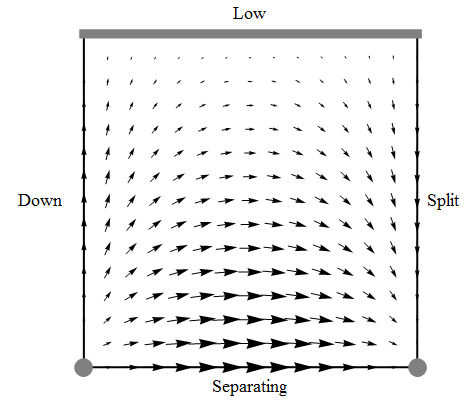
\includegraphics[scale=.4]{Graph16}}
\hfill
\subfloat[$K=.5$]{\label{fig:Graph17.png}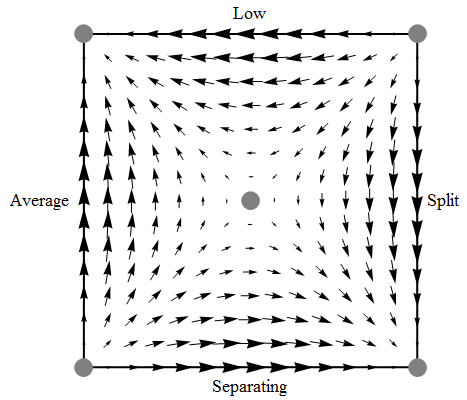
\includegraphics[scale=.4]{Graph17}}
\end{center}
\caption{Phase space for two values of $K$ with $C=.5$ and $P_H=.5$}
\label{fig:Graph16.png and fig:Graph17.png}
\end{figure}

We again find a mixed equilibrium, in the shape of a saddle point, which appears within the boundaries of phase space for particular values of our parameters. Although it is tempting to say that the graphs are different for various values of the parameters, there is again only one fundamental dynamic of this model. The (Low, Average) and (Separating, Split) combined strategies are basically always equilibria, although the proportion of phase space which is attracted to these endpoints varies with the parameters. These parameters also determine whether there is a mixed equilibrium within phase space. It turns out that the position of the saddle point is given by similar equations as before.

\begin{subequations}
\label{eq:Position2D-12}
\begin{equation}
{x_1}=\frac{K^2+P_H-2 K P_H}{P_H}
\end{equation}
\begin{equation}
{y_1}=1-C
\end{equation}
\end{subequations}

It is useful to do the same analysis on another part of the model's phase space by restricting the strategies to Separating or High and to Average or Split. This means we are looking at the boundary face for which $x_1=0$.
 
\begin{figure}[h]
\begin{center}
\subfloat[$K=0$]{\label{fig:Graph18.png}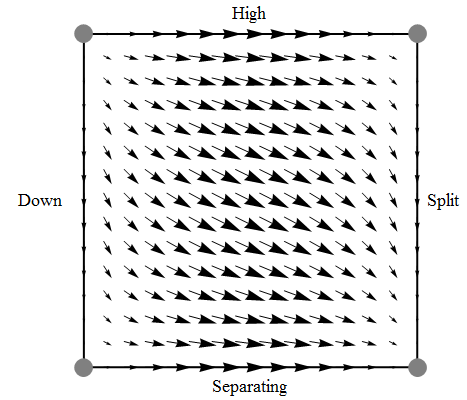
\includegraphics[scale=.4]{Graph18}}
\hfill
\subfloat[$K=.5$]{\label{fig:Graph19.png}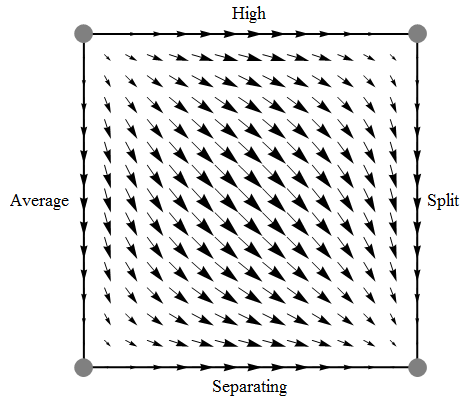
\includegraphics[scale=.4]{Graph19}}
\end{center}
\caption{Phase space for two values of $K$ with $C=.5$ and $P_H=.5$}
\label{fig:Graph18.png and fig:Graph19.png}
\end{figure}

In this case, we do not find a mixed equilibrium. In fact, if we try to solve the equations for the positions of the mixed equilibrium, we find no answer. There is no mixed equilibrium for any value of $P_H$ or $S$. We see that for all cases, the (Separating, Split) combined strategy is the Nash equilibrium to which all initial configurations evolve. Here, all low quality senders will choose not to reveal their goods because there is a cost associated with revelation, however, receivers will interpret their hiding as a sign of low quality. Likewise, high quality senders will find it advantageous to reveal, because this means they will be awarded the higher revenue.\\
\\
Finally, these strategies can again be put together in a three dimensional phase space, as presented below in Figure~\ref{fig:Graph20.png}. As before, we have a situation in which the sender can choose High, Low or Separating and the receiver can choose Average or Split.

\begin{figure}[h]
\begin{center}
\leavevmode
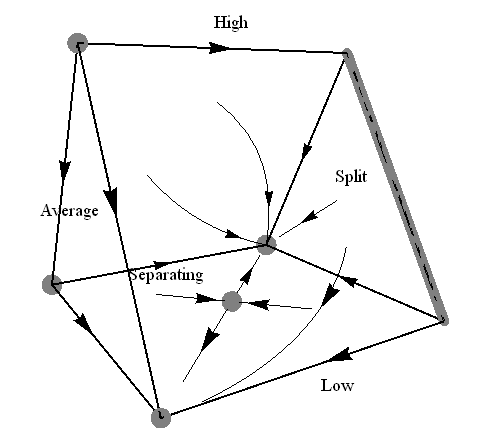
\includegraphics[scale=.75]{Graph20.png}
\end{center}
\caption{Three dimensional phase space with $K=.5$, $P_H=.5$ and $C=.5$.}
\label{fig:Graph20.png}
\end{figure}

What we find here is interesting. In comparison to the dynamics of costly signalling, these dynamics turn out to be simpler. There is no attractive mixed equilibrium, only a saddle point which splits phase space into two parts for which either the (Low, Average) combined strategy is the final end point or for which (Separating, Split) will be the stable equilibrium. The first equilibrium corresponds to a situation in which no-one reveals and the receiver pays an averaged revenue. The second to a situation in which only high quality senders reveal and get paid the high revenue and where low senders hide their quality, resulting in the low revenue.

\section{Conclusion}
\label{sec:Conclusion}
\subsection{Costly Signalling}
\label{sec:Costly Signalling}

We have looked at Spence's model and have tried to determine what the dynamics of this model would be under various values for its parameters. In particular, we have taken Wagner's model under examination which had drawn some attention for having suggested the importance of mixed equilibria in these signalling models. In a mixed equilibrium, a proportion of the players chooses one strategy, while others players choose a different strategy. As such, these states of the model are only partially communicative, allowing receivers to discriminate between the groups of senders only up to a certain point. It was suggested that a possible reason for the lack of previous accounts of mixed equilibria was that these only occur when the pooling, averaged revenue $\rho_A$ was sufficiently different from both $\rho_U$ and $\rho_D$. To show this, we have calculated the position of the mixed equilibria as a function of our parameter $K$, which allows us to scan $\rho_A$ from 1 to 2.\\
\\
The possibility for a varying $K$ is very similar to an infinite strategy space for the receiver, however, the difference was that we set $K$ globally for all receivers. It would be interesting to see what the dynamics would be if $K$ was really allowed to vary, but this is left for further research. One possible result would be that all receivers would converge to a specific value for $K$. Following the assumption that receivers wish to minimize the difference between the paid revenue and the received marginal product, it must be the case that there is an optimal value for $K$ which succeeds in this. In fact, as we have seen, the pay-off to the receiver under the Average strategy is $-P_H (1-K)^2-P_L K^2$. This pay-off is maximized when $K=P_H$, which results in $\rho_A$ being precisely equal to the expected marginal product of all senders,  $1+P_H$. Underlining the importance of mixed equilibria, this idea suggests that in the real world, where receivers often do possess an infinite strategy space, mixed equilibria evolve naturally due to the receivers maximizing their pay-offs and choosing a value of $K$ equal to the proportion of high quality senders, $P_H$. This is also the value which Wagner chose for his pooling strategy and it is clearly a very reasonable averaged revenue, which stands at the heart of the existence of mixed equilibria.\\
\\
However, the existence of a mixed equilibrium on a boundary face of Spence's model was also shown to be independent of the values of the parameters of the model in some way. The mixed equilibrium is always there, but it may not lie within phase space. Its coordinates depend on the parameters and, therefore, the dynamics of the model depend on the parameters as well. It is important to realise that there are not many fundamentally different dynamics on these phase spaces. As we have seen, varying the parameters causes the position of the mixed equilibrium to shift which then shows us a different part of a larger dynamic within the boundaries of phase space. In extreme cases, this may lead to changes in the stability of pure-strategy equilibria, but the larger picture is always fundamentally the same. The main point which Wagner's model shows us is that partially communicative mixed equilibria are possibly more the norm rather than the exception \cite{Wagner2010}. It is precisely because of the cost of signalling that Spence's model can create a situation in which receivers can perfectly discriminate between low and high quality, but when evolution or learning comes into play, it may be the case that mixed equilibria are simply more likely results. When one looks at nature, both in the world of economics as well as in biology, it is not surprising to find only partially communicative equilibria. For example, in the job market education cannot be viewed as a perfectly communicative signal. Furthermore, we often find boom and bust cycles in nature, which may be closely related to the limit cycle found in Wagner's model, where both wages and level of education go up and down with time.

\subsection{To Reveal or Not to Reveal}
\label{sec:To Reveal or Not to Reveal}

One aspect of Wagner's model which may still cause it to run into criticism is the fact that it relies heavily on pruning. Remember that the sender has potentially four strategies to play, while the receiver has nine. The combinations of these strategies would result in a phase space which is much too large to analyse, while there are clearly parts which are not even interesting for analysis. However, to assume that the pruned version of the model is fully without loss of generality may be risky. As we had already mentioned, it becomes easier to argue for pruning when one is dealing with revelation. Under revelation, the sender shows his type to the receiver, who can then decide what revenue to award the sender. Clearly a receiver, who wishes to minimize the difference between the awarded revenue and the received marginal product, would not choose any strategy in which he pays a sender a revenue not equal to his marginal product when he can perfectly see the sender's type. Therefore, even though the number of possible strategies for the receiver is larger, the pruning becomes easier and only a few reasonable strategies remain. One of these strategies was called Split, where the receiver paid the high and the low revenue to these types when they revealed to him and where he paid the low revenue to a sender who was hiding his type. The receiver, then, considered hiding a sign of low quality and it was shown that, in combination with the senders' strategy Separating, this formed a stable Nash equilibrium. In that case, low quality senders would not reveal when there was a cost associated with revelation and would accept the lower revenue, while high quality senders would reveal their type, if the cost was not too large, and would receive a higher pay-off.\\
\\
The dynamics of revelation ended up being simpler than those for costly signalling as well. Even though there was a saddle point on one boundary face of the three dimensional phase space, there was no stable, attractive mixed equilibrium like in the case of Wagner's model. The dynamics showed that the (Separating, Split) combined strategy was the most likely end point for a population of senders and receivers who wished to maximize their pay-off. However, under certain conditions the (Low, Average) combined strategy could also attract a large proportion of phase space. In that case, receivers would not be influenced by revelation and would pool all types of senders into one group, paying them an averaged revenue. The senders would then choose not to reveal at all, because there was a cost associated with revelation, while no additional benefit awaited them.\\
\\
When revelation was cheap, low quality senders would see no disadvantage in revealing their type, as the awarded revenue would be the same. The dynamics would, therefore, not change dramatically. This is in contrast to cheap signalling, which relies on aligned preferences of the senders and receivers and which is fundamentally different from the case of costly signalling. When signalling is cheap, lying is prominent in the case of non-aligned preferences. However, for revelation, the cost of revelation has little influence on the decisions of the receiver. In most cases, he would pay a sender who did not reveal the low revenue, rightfully assuming he was of low quality. In a strong analogy to Spence's model, we can conclude that the question of whether to reveal or not to reveal depends fully on the type of the sender, in such a way that receivers can fully discriminate between high quality and low quality senders.

\newpage

\phantomsection
\label{sec:Bibliography}
\addcontentsline{toc}{section}{Bibliography}
\renewcommand{\refname}{Bibliography\\} 
\bibliographystyle{plain}
\bibliography{Bibliography}

\newpage

\appendix
\label{sec:Appendix}
\section{Appendix}

\subsection{Pay-Off Matrix Calculations}
\label{sec:Pay-Off Matrix Calculations}

This section will briefly explain how the expected pay-offs for a particular strategy are determined. As can be seen in Table~\ref{tab:PayoffMatrix3D1}, the pay-off to a sender who plays High, under the receiver's strategy Average, is $1+K-\frac{1}{2}P_H S-P_L S$. We identify three parts in this expression. The first is $1+K$ which is equal to the revenue $\rho_A$ awarded by the receiver. The second part is $\frac{1}{2}P_H S$. The cost incurred by high quality senders for signalling is $\frac{1}{2}S$ and seeing there are $P_H$ of these senders, this will be the cost incurred by all of them. The same argument goes for the $P_L$ low quality senders who incur a cost equal to $S$, resulting in the expression above. For the other strategies, the awarded revenue differs and the total costs incurred from signalling changes depending on the number of player who signal, however, the basic calculation is the same. For the receiver, the pay-off is determined by the quadratic difference between the revenue he pays and the marginal product he gets. Under (High, Average), he obtains $P_H$ high quality senders who are worth 2 to him. As he pays them $1+K$, the difference is $1-K$. The cost for this group of senders becomes $P_H{(1-K)}^2$. For the low quality senders, the calculation is the same, with a quadratic difference between the revenue $\rho_A$ and 1 of ${K}^2$. The total pay-off to the receivers, then, is $-P_H (1-K)^2-P_L K^2$. For the other combined strategies, the revenues again differ, but the method of calculation is still fundamentally the same.

\subsection{The Replicator Equation}
\label{sec:The Replicator Equation}

We have been considering a population of senders and receivers who play the signalling game and obtain pay-offs. For simplicity, it is assumed the population is infinitely large. We denoted different players with different strategies as $x_1$, $x_2$, $x_3$. Now, we wish to find a law of motion which describes the evolution of these numbers in time $t$. We then view these proportions as elements of vector $x(t)$. If two players are randomly assigned to play the game, the expected pay-off of player type $i$ would be ${(Ax)}_i$, where $A$ denotes the pay-off matrix. For the whole population, the average pay-off is then given by $x^T Ax$. Let us assume that the rate of growth, which is given by $\frac{\dot{x}_i}{x_i}$, is equal to the difference between the pay-off for player type $i$ and the average pay-off in the population. This yields the replicator equation \cite{Hofbauer2003}.

\begin{equation}
\label{eq:Replicator}
\dot{x}_i=x_i({(Ax)}_i-x^T Ax)
\end{equation}

This non-linear differential equation is most easily solved numerically. For this paper, the computer programme \textit{Mathematica} was used to solve the equation. Specific solutions were then plotted to obtain the graphs used in this paper.

\subsection{Mixed Equilibria}
\label{sec:Mixed Equilibria}

The condition which must be satisfied for a mixed equilibrium to exist is that, for a particular proportion of strategies among the players, there is no incentive for any player to change his strategy. This must hold for both the senders and the recievers. In the two dimensional phase space we have often considered above, if we have $x_1$ senders choosing strategy Low, there are $1-x_1$ senders choosing Separating. Likewise, if there are $y_1$ receivers playing Average, there will be $1-y_1$ receivers choosing Split. A mixed equilibrium will then exist if the pay-off to the first group of players is the same as the pay-off to the second group of players, for both senders and receivers \cite{Gintis2009}.

\begin{subequations}
\label{eq:Solvexandy}
\begin{equation}
{(Ay)}_1={(Ay)}_2
\end{equation}
\begin{equation}
{(Bx)}_1={(Bx)}_2
\end{equation}
\end{subequations}

In these equations, $x(t)$ and $y(t)$ are again vectors composing of the elements $x_1$ and $1-x_1$, and $y_1$ and $1-y_1$. Furthermore, $A$ and $B$ are the pay-off matrices for the senders and receivers, respectively. It is easy to solve these equations for $x_1$ and $y_1$, if a mixed equilibrium exists.

\subsection{The Strategies for Revelation}
\label{sec:The Strategies for Revelation}

The strategies which are possible for the receiver in the revelation model are more than those available under costly signalling. Now, there are not 9 strategies, but $3\cdot9=27$ strategies. The reason for this is that, when a sender reveals his type, the receiver can act differently for high and for low types. This gives him another dimension to act in, resulting in a list of three columns of permutations of the options Up, Average and Down. However, only a few of them are reasonable, because it would not make sense for a receiver, for example, to award a low quality sender, who has revealed his type to the receiver, with a revenue $\rho_U$. The list below shows the strategies for the sender and all 27 possible strategies for the receiver, with names for only a few of them.

\begin{table}[h]
\begin{center}
\begin{tabular}{c|c|ccc|c|c|c}
\multicolumn{2}{c|}{Response to}&Name& \hspace{1cm} &\multicolumn{3}{c|}{Response to}&Name\\
High&Low&&&West&\multicolumn{2}{c|}{East}&\\
&&&&&High&Low&\\
\cline{1-3}
\cline{5-8}
&&&&&&\\[-.3cm]
E&E&High/Always Reveal&&U&U&U&Always Up\\
E&W&Separating&&U&U&A&-\\
W&E&Anti-Separating&&U&U&D&-\\
W&W&Low/Never Reveal&&U&A&U&-\\
\multicolumn{3}{c}{}&&U&A&A&-\\
\multicolumn{3}{c}{}&&U&A&D&-\\
\multicolumn{3}{c}{}&&U&D&U&Anti-Split\\
\multicolumn{3}{c}{}&&U&D&A&-\\
\multicolumn{3}{c}{}&&U&D&D&-\\
\multicolumn{3}{c}{}&&A&U&U&-\\
\multicolumn{3}{c}{}&&A&U&A&-\\
\multicolumn{3}{c}{}&&A&U&D&-\\
\multicolumn{3}{c}{}&&A&A&U&-\\
\multicolumn{3}{c}{}&&A&A&A&Always Average\\
\multicolumn{3}{c}{}&&A&A&D&-\\
\multicolumn{3}{c}{}&&A&D&U&-\\
\multicolumn{3}{c}{}&&A&D&A&-\\
\multicolumn{3}{c}{}&&A&D&D&-\\
\multicolumn{3}{c}{}&&D&U&U&-\\
\multicolumn{3}{c}{}&&D&U&A&-\\
\multicolumn{3}{c}{}&&D&U&D&Split\\
\multicolumn{3}{c}{}&&D&A&U&-\\
\multicolumn{3}{c}{}&&D&A&A&-\\
\multicolumn{3}{c}{}&&D&A&D&-\\
\multicolumn{3}{c}{}&&D&D&U&-\\
\multicolumn{3}{c}{}&&D&D&A&-\\
\multicolumn{3}{c}{}&&D&D&D&Always Down\\
\end{tabular}
\end{center}
\caption{Strategies of the senders and receivers}
\label{tab:StrategiesRevelationFull}
\end{table}

\end{document}